\section{Grafické prostředí}
\paragraph{}
Grafické prostředí na této stránce je rozděleno do dvou základních šablon. Tyto šablony jsou různě modifikovány. Stránky mají konzistentní jednoduchý desing a tak jsou snadno zapamatovatelné a uživatel se v nich rychle zorientuje. Díky jednoduchému desingu bylo docíleno responzivní verze pouze s minimálnímy zásahy do originální počítačové verze. 
\subsection{Úvodní část}
\subsubsection{Přihlašovací stránka}
\paragraph{} 
Přihlašovací obrazovka byla zvolena jednotná pro administrátora i pro uživatele. Styl, který byl použit byl co nejjednoduší to šlo. Je to hlavní strana aplikace. Všechno tu má svůj význam a cíl. Stránka není myšlena jako stránka, na které by se člověk zajímal o tuto aplikaci, naopak je myšlena na už znalého uživatele, který jde na tuto stránku s jasným cílem a to přihlásit se nebo se registrovat. 
\begin{figure}[h]
\centering
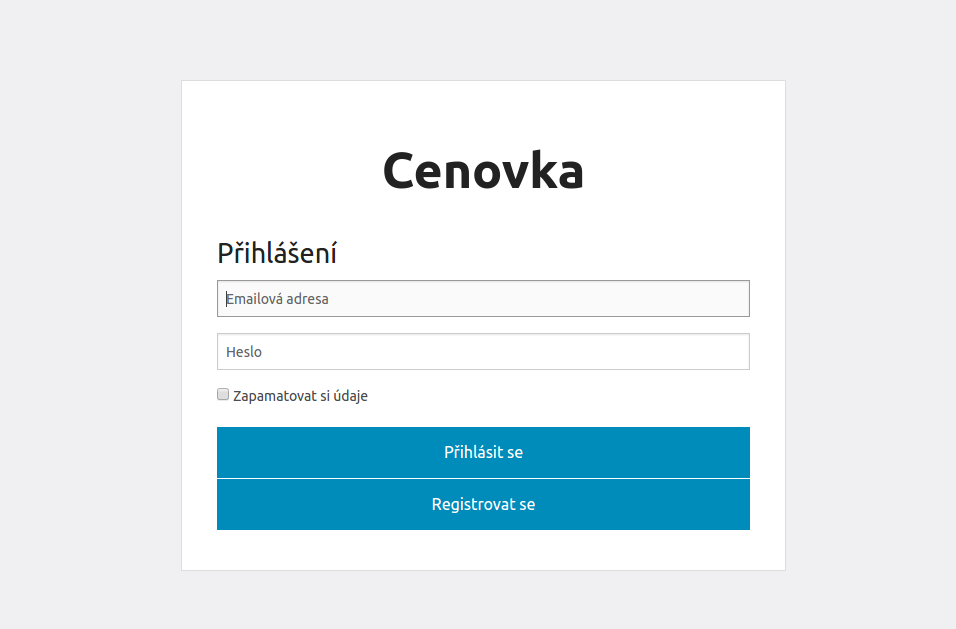
\includegraphics[width=1\textwidth]{graphic/login.png}
\caption{Přihlašovací formulář}
\end{figure}
\paragraph{} 
Celý obsah je zarovnaný do prostřed stránky, jak vertikálně, tak horizontálně, a zmenšený pouze na nezbitnou šířku a výšku. Nad dvěmi poli pro přihlášení leží nadpisy stránek. Pod poli leží zaškrtávací tlačítko pro dlouhodobé přihlášení. Dále tu leží tlačítko na přihlášení a poté tlačítko, které vás přesměrovává na formulář s registrací. 
\subsubsection{Registrační stránka}
\paragraph{}
Registrační formulář se nese ve stejném stylu, jako stránka přihlašovací. Jeji obsah je znovu vystředěný horizontálně i vertikálně, nyní je ale lehce vyšší. Tím, že přihlášení a registrace nejsou zatíženy žádnými dalšími informacemi působí to, jako vstupní brána, která izoluje aplikaci od stránek, z kterých uživatel přichází.
\begin{figure}[h]
\centering
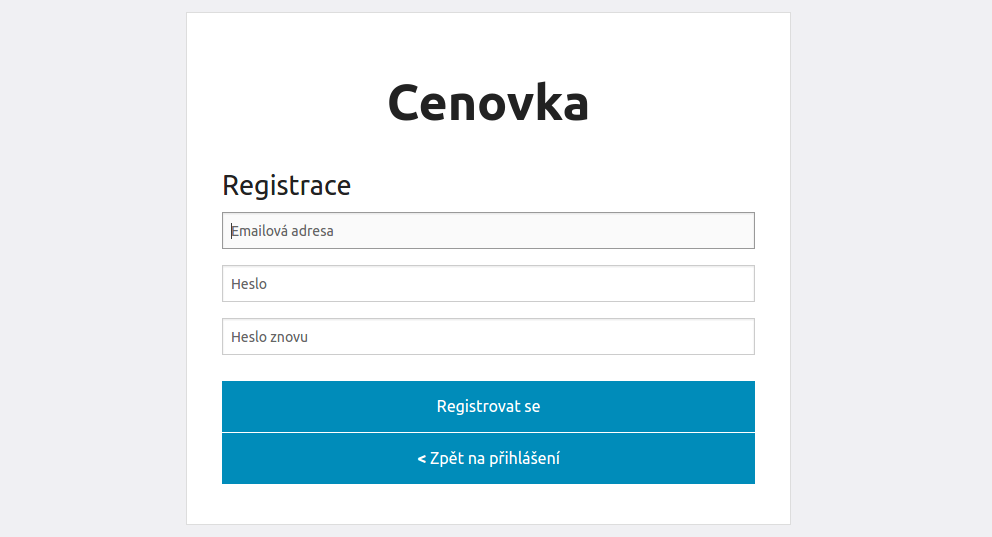
\includegraphics[width=1\textwidth]{graphic/register.png}
\caption{Registrační formulář}
\end{figure}

\subsection{Oznamovací oblast}
Cokoli se stane o čem by měl uživatel vědět, tak je zobrazeno obdelníkem se zprávou v pravé spodní části. Tato komponenta je společná pro celou stránku. 
\begin{figure}[h]
\centering

\includegraphics[width=1\textwidth]{graphic/alert.png}
\caption{Oznamovací Oblast}
\end{figure}
